\documentclass[onecolumn, draftclsnofoot,10pt, compsoc]{IEEEtran}
\usepackage{graphicx}
\usepackage{url}
\usepackage{setspace}


\usepackage{geometry}
\geometry{textheight=9.5in, textwidth=7in}

% 1. Fill in these details
\def \CapstoneTeamName{		The Cleverly Named Team}
\def \CapstoneTeamNumber{		12}
\def \GroupMemberOne{			Quanah Green}
\def \GroupMemberTwo{			Alex Ruef}
\def \GroupMemberThree{			Ethan Takla}
\def \CapstoneProjectName{		Remote Seed Identification}
\def \CapstoneSponsorCompany{	Crop and Soil Science Department, OSU}
\def \CapstoneSponsorPerson{		Dan Curry}

% 2. Uncomment the appropriate line below so that the document type works
\def \DocType{		%Problem Statement
				Requirements Document
				%Technology Review
				%Design Document
				%Progress Report
				}
			
\newcommand{\NameSigPair}[1]{\par
\makebox[2.75in][r]{#1} \hfil 	\makebox[3.25in]{\makebox[2.25in]{\hrulefill} \hfill		\makebox[.75in]{\hrulefill}}
\par\vspace{-12pt} \textit{\tiny\noindent
\makebox[2.75in]{} \hfil		\makebox[3.25in]{\makebox[2.25in][r]{Signature} \hfill	\makebox[.75in][r]{Date}}}}
% 3. If the document is not to be signed, uncomment the RENEWcommand below
\renewcommand{\NameSigPair}[1]{#1}

%%%%%%%%%%%%%%%%%%%%%%%%%%%%%%%%%%%%%%%
\begin{document}
\begin{titlepage}
    \pagenumbering{gobble}
    \begin{singlespace}
    	%\includegraphics[height=4cm]{coe_v_spot1}
        \hfill 
        % 4. If you have a logo, use this includegraphics command to put it on the coversheet.
        %\includegraphics[height=4cm]{CompanyLogo}   
        \par\vspace{.2in}
        \centering
        \scshape{
            \huge CS Capstone \DocType \par
            {\large\today}\par
            \vspace{.5in}
            \textbf{\Huge\CapstoneProjectName}\par
            \vfill
            {\large Prepared for}\par
            \Huge \CapstoneSponsorCompany\par
            \vspace{5pt}
            {\Large\NameSigPair{\CapstoneSponsorPerson}\par}
            {\large Prepared by }\par
            Group\CapstoneTeamNumber\par
            % 5. comment out the line below this one if you do not wish to name your team
            %\CapstoneTeamName\par 
            \vspace{5pt}
            {\Large
                \NameSigPair{\GroupMemberOne}\par
                \NameSigPair{\GroupMemberTwo}\par
                \NameSigPair{\GroupMemberThree}\par
            }
            \vspace{20pt}
        }
        \begin{abstract}
		In this document, the hardware and software requirements are defined in detail in order to ensure the timely completion of the remote seed identification project. The project will have a basic minimum set of goals with a set of stretch goals if research goes favorably. 

        \end{abstract}     
    \end{singlespace}
\end{titlepage}
\newpage
\pagenumbering{arabic}
\tableofcontents
% 7. uncomment this (if applicable). Consider adding a page break.
%\listoffigures
%\listoftables
\clearpage

\section{Introduction}
\subsection{Purpose}
In this document we outline in detail the software and hardware requirements for the Remote Seed Identification project. The requirements and their respective time-lines will be used to guide this project and its development, and additionally to unify the expectations of the project between Daniel Curry of the OSU Seed Lab and Capstone group 12. 

\subsection{Scope}
The software to be developed will have three main components for the remote seed identification; a mobile Android application, a dedicated web server that allows the client to send and receive data from the Jetson TX2, and the seed identification algorithm that will do most of the important processing. The current seed identification process is very slow, and this software application will help to significantly reduce seed analysis times and let researchers spend their time on more important work. Due to the fact that the grass seed industry is quite small, there hasn't been a big effort to automate grass seed analysis, meaning the end product could have huge implications. Due to the novel nature of this project, a set of basic minimum functionality will be defined, following a set of ultimate stretch goals.  
\subsection{Definitions}
\begin{itemize}
\item
\textbf{Sample: } This refers to a sample of seeds, which will typically be 500 seeds in size. If the project completes its ultimate ambitions, the sample will be 2500 seeds
\item
\textbf{NVIDIA Jetson TX2: } This is a power processor aimed at artificial intelligence and machine learning applications. This is what will run computationally intensive tasks in our back end
\item
\textbf{Open Source Computer Vision Library (OpenCV): } An extensive, highly tested computer vision library optimized to run on NVIDIA processors.
\item
\textbf{Deep Neural Network (DNN): } This refers to one of OpenCV's many features, and is the main component behind the seed identification algorithm.
\end{itemize}


\section{Overall Description}
\subsection{Product Perspective}
This project aims to reduce manual seed analysis in both Oregon State Seed labs and in the field. The introduction of a simple, quick way to analyze seeds will remove a significant bottleneck that has been frustrating scientists for years.
Rather than sending the seed samples to a lab, users will send images of samples to be processed using the Jetson TX2 through a dedicated Android application.
Users will be able to view and quantify important results such as how pure the sample is, and if the stretch goals are met should be able to correctly identify and localize seed species in the sample.
The application itself will be extremely user-intuitive, enabling individuals with no prior experience to master the process in a few simple steps.


\subsection{Product Functions}

As previously mentioned, the remote seed identifier will be split up into three main components: the client-end application, a web server used for sending and receiving data, and the back-end processing unit using. 

The client-end android application will be developed as an android application, and will allow the user to easily send pictures of seed samples and get results in minutes. The client application will guide users on how to take a proper image of a sample, and alert them when their results are ready for analysis. The quality analysis generated for the client will greatly depend on whether the team is able to over-come the issue of low resolution phone and tablet cameras. Additionally, clients will have to make accounts and be approved by an administrator in order to use the seed identification service.

The web server will be constantly running on the Jetson TX2, ready and waiting to accept sample jobs and process them. The web server will only accept jobs that come from registered and approved clients using the app. 

Once data is received via the web server on the Jetson TX2, DNN's image classification will be used to analyze seed samples. OpenCV is optimized to run on the Jetsons 256-core processor, so the results will be able to be generated with low latency. Due to the possible performance restrictions associated with low-resolution cameras, the basic minimum requirement for the seed identifier is that it can find rogue seeds in the sample and determine how pure the sample is depending on how many seeds it finds total. As a stretch goal, the algorithm should be able to correctly identify seed species as well, which would be beneficial information to seed analysts. Additionally, since it is difficult to count seeds by hand, the number of seeds in the sample will be automatically counted by the software. 

\subsection{User Characteristics}
Target users of this tool will primarily be college students and seed analysts, although the intention is for to be usable by anyone that picks up the application. Seed analysts will typically be handling high numbers of samples per day, and need a quick efficient way to view the statistics on their samples. As far as mobile devices, a user will usually be using an iPhone or Android device with camera resolutions as low as 5 megapixels for older devices. 

\subsection{Constraints}
A NVIDIA Jetson TX2 processor will be used to do the image analysis.
The power of the Jetson will directly impact the processing time and the format of the input images. Additionally, since many people will be using this app, the phone camera resolution of the devices will vary significantly.The resolution of the input images will directly effect the accuracy of the seed identification software. 

\subsection{Assumptions and Dependencies}
The assumption is made that the average phone camera will have high enough resolution to obtain high accuracy for identifying if a seed is rogue. If a good phone is used, the goal is to also identify the species of the rogue seed as well. 

\subsection{Apportioning Requirements}
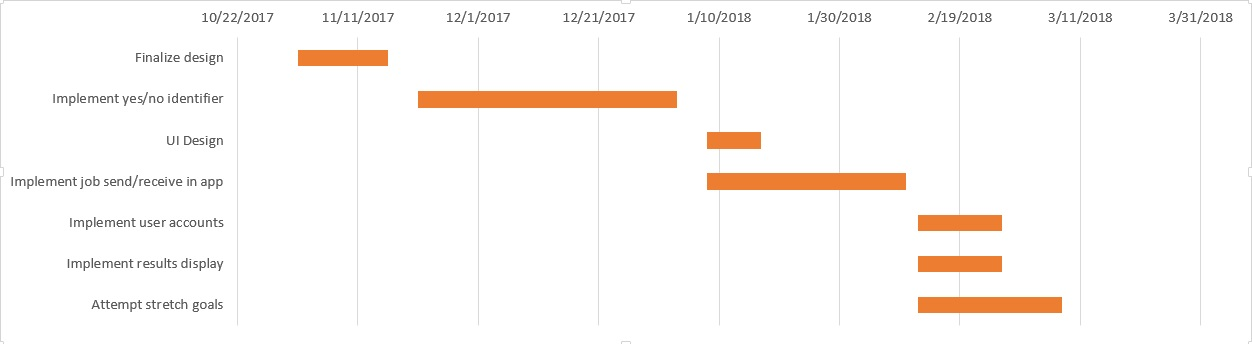
\includegraphics[scale=0.65]{gantt_chart.jpg}

\section{Specific requirements}
This section describes in detail the basic minimum set of requirements, as well as stretch goals to be reached as well. 

\subsection{Functions}
\begin{itemize}
\item
\textbf{Minimum requirements}
\begin{enumerate}
\item
When taking pictures of the samples, a user should be able to optionally have easy to understand instructions on how to take good photos of the samples. 
\item
A user should have regular in-app feedback on the status of the seed processing job so that they know the system is working properly. 
\item
A user should be able to save and label analysis results within the application so that they can view the results later. This includes both the image of the sample and the report
\item
A user should be able to send analysis results (including saved ones) via email in a PDF format
\item
A user should be able to send an image of a 500 seed sample to be processed using the app. 
\item
A user should receive a notification on their mobile device when their sample has been processed. 
\item
A user should be able to view an image of the sample which details the location of the rogue seeds so that they can remove them.
\item
A user should be able to view the percentage of rogue seeds in the results so that they can get a estimate on the quality of the sample.
\item
Due to the difficulties of counting out exactly 500 seeds, a user should be able to view the number of seeds that were in the sample in the results
\end{enumerate}
\item
\textbf{Ultimate ambitions}
\begin{enumerate}
\item
A user should be able to view the species of each rogue seed in the sample so that they can get a better idea of the seeds contaminating the sample. 
\item
A user should be able send an image of a 2500 seed sample to be processed. 
\item
An organization should be able to archive all reports made by analysts, so that they can use them at a later time if needed. 
\end{enumerate}
\end{itemize}

\subsection{Performance and Reliability Requirements}
\begin{enumerate}
\item
Due to the fact that this project is slightly a research one in nature, it would be almost impossible to estimate what the performance requirements should be. A reasonable goal for the basic seed identifier would be a 95 percent accuracy of the purity of the sample. 
\end{enumerate}
\subsection{Standards Compliance}
\begin{enumerate}
\item
A user analyst should be able to view the confidence level the identifier had in the sample, meaning the results can be discarded if it doesn't meet the confidence threshold defined by system administrators. This allows organizations to define their own standards for what results they can and cannot use.
\end{enumerate}
\subsection{Availability}
\begin{enumerate}
\item
A user should be available to use the service 24/7, or as long as Oregon State's networks are working properly, to make the system as flexible as possible for users.
\end{enumerate}
\subsection{Security}

\begin{enumerate}
\item
A user should be able to create an analyst account with a password and user name within the mobile application so that they can gain access to the identification service.
\item
A user account can be given administrator permissions in order to allow organizations to control who gets to use the service. 
\item
Administrators are able to approve accounts for usage. This gives a high level of control of who can use the system.
\end{enumerate}

\subsection{Maintainability}
\begin{enumerate}
\item
As a stretch goal, a user should be able to upload images of seeds species that currently aren't supported by the app to be trained.
\end{enumerate}
\subsection{Portability}
\begin{enumerate}
\item
A user should be able to download the application on an Android device. As a stretch goal, the app will also be supported on iOS.
\end{enumerate}

\end{document}
